\section{Technical Overview}

\begin{figure*}[t]
\centering
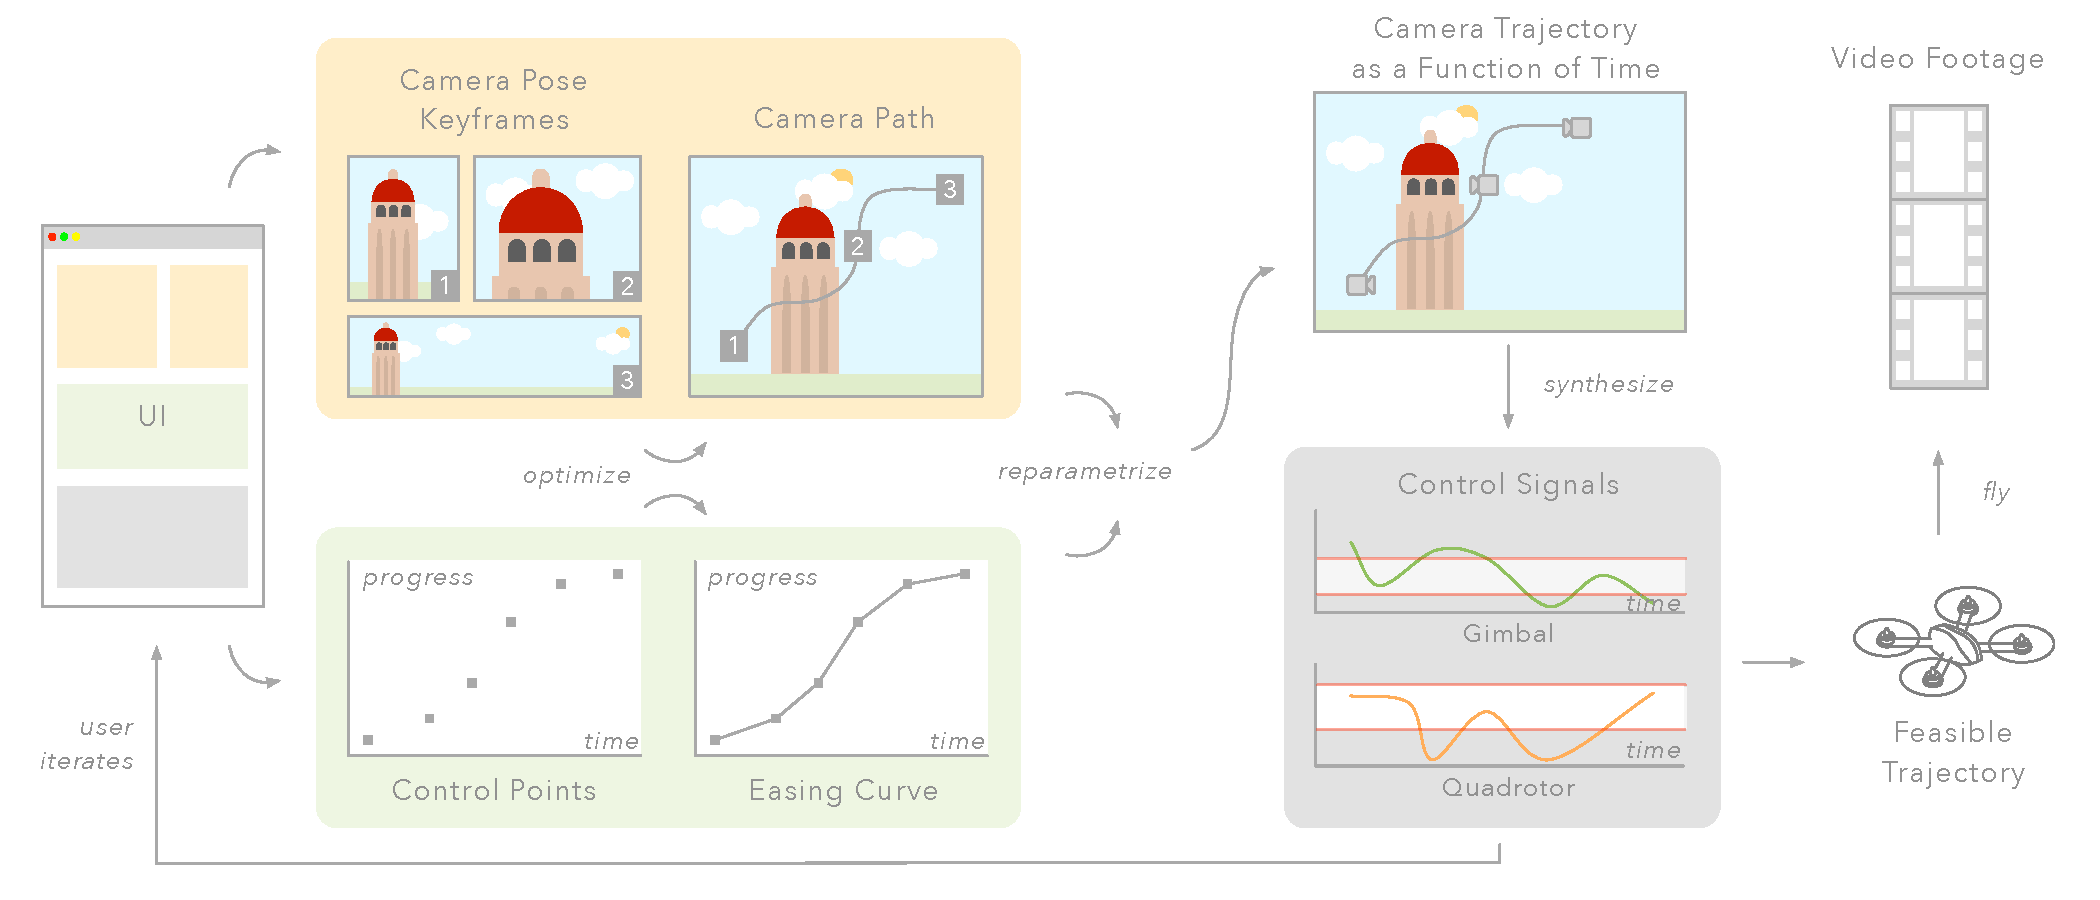
\includegraphics[width=6.0in]{images/2015_siggraph_asia/system_overview}
\caption{
Overview of the major technical components of our system.
We begin with two user-specified inputs: (1) camera pose keyframes in a virtual environment (e.g., \textsc{Google Earth}); and (2) a sequence of easing curve control points.
From these inputs, we compute a smooth camera path and a smooth easing curve.
We optimize the smoothness of the camera path and easing curve in a way that obeys the physical equations of motion for quadrotors.
We re-paramterize the camera path, according to the easing curve, to produce a camera trajectory as a function of time.
We synthesize the control signals required for a quadrotor and gimbal to follow the camera trajectory.
We plot these control signals in our user interface, providing the user with visual feedback about the physical feasibility of the resulting trajectory.
The user can edit the resulting trajectory by editing camera pose keyframes and easing curve control points.
Once the user is satisfied with the trajectory, we command a quadrotor camera to execute the trajectory fully autonomously, capturing real video footage.
}
\label{figure:overview}
\end{figure*}

We provide an overview of the major technical components of our system in Figure~\ref{figure:overview}.
At the core of our system is a physical quadrotor camera model, in which a rigid body quadrotor is attached to a camera mounted on a gimbal (Section~\ref{sec:ch2:model}).
In this model, the quadrotor and the gimbal are physically coupled, which enables us to consider their motion jointly.

We analyze the dynamics of our model, and show that camera trajectories must be $C^4$ continuous in order to obey the physical equations of motion for quadrotors.
With this requirement in mind, we derive an algorithm for synthesizing $C^4$ continuous camera trajectories from user-specified keyframes and easing curves (Section~\ref{sec:ch2:synthesizing_virtual_camera_trajectories}).
This algorithm enables users to design shots visually, and gives users precise control over the timing of their shot.
At a high level, our approach is to optimize the smoothness of the camera trajectory by solving a constrained quadratic minimization problem that guarantees $C^4$ continuity.

We then derive an algorithm to compute the control signals required for a quadrotor and gimbal to follow any $C^4$ continuous camera trajectory (Section~\ref{sec:ch2:flatness}).
This algorithm enables our tool to provide the user with visually accurate shot previews, and visual feedback about the physical feasibility of camera trajectories.
At a high level, our approach is to compute a trajectory through our quadrotor camera's state space that places the gimbal at the same world frame pose as the camera we are trying to follow at all times.
We use this state space trajectory to solve for the quadrotor and gimbal control signals.

Our algorithm for synthesizing camera trajectories is guaranteed to produce trajectories that obey the physical equations of motion for quadrotors.
However, our algorithm might produce trajectories that exceed the physical limits of a particular real-world quadrotor.
As discussed in Section~\ref{sec:ch2:ui}, our strategy for handling these physically infeasible trajectories is interactive.
%We compute dynamic and kinematic quantities of interest along the user's intended camera trajectory (e.g., gimbal joint angles, velocities, and thrust forces), and display these quantities to the user on a set of feasibility plots.
%Based on this visual feedback, the user can adapt her shot to the physical limits of her hardware.

Once the user is satisfied with her camera trajectory, we command a quadrotor camera to execute the trajectory fully autonomously, capturing real video footage (Section~\ref{sec:ch2:hw}).
At a high level, we use the camera trajectory computed in Section~\ref{sec:ch2:synthesizing_virtual_camera_trajectories} to drive a feedback controller running on a real-world quadrotor.
This feedback controller compensates for unexpected disturbances, unmodeled forces, and sensor noise, without having to explicitly re-compute the camera trajectory.
We execute the user's intended camera trajectory by sampling the position and velocity of look-at and look-from points along the trajectory, and transmitting these quantities to the quadrotor.
%This feedback controller takes as input the position and velocity of look-at and look-from points along the intended camera trajectory.
Strictly speaking, we could attempt to execute the camera trajectories computed in Section~\ref{sec:ch2:synthesizing_virtual_camera_trajectories}, without going to the extra trouble of  computing control signals  in Section~\ref{sec:ch2:flatness}.
However, computing control signals enables our tool to provide visual feedback about the physical feasibility of trajectories, which is an important safety feature. Moreover, computing control signals enables our tool to \emph{certify} the accuracy of visual shot previews, since the visual preview will be accurate only if the trajectory is physically feasible.

\begin{tcolorbox}[before skip=20pt, after skip=20pt, sharp corners]
\begin{center}
\textbf{In the following chapter, we will \emph{computationally} generate trajectories that adhere to the physical limits of a quadrotor.}
\textbf{But for now, we rely on the user to adjust her shot if it violates these limits.}
\end{center}
\end{tcolorbox}

